%Depracted
\newcommand{\mrN}{\mathrm{N}}
\newcommand{\mrS}{\mathrm{S}}
\newcommand{\mrE}{\mathrm{E}}
\newcommand{\mrW}{\mathrm{W}}


\section{The red algo}
\paragraph{Notational concerns}
We will use $\C$ to indicate the current sweep line cycle.
We will repeatedly only consider the path $\cpath$. In that case we will always order it from $\mrW$ to $\mrE$.

We will let $\W$ denote a interior walk  \fxnote{have i defined this already}. Given such a walk of $k$ vertices we index it's nodes $w_1, \ldots, w_k$  in such a way that $w_1$ is closer to $W$ then $w_k$ is (and thus that $w_k$ is closer to $E$ then $w_1$ is).

Then $w_1$ and $w_k$ indicate the two unique vertices of the walk that are also part of the cycle. We will then let $\restC{\W}$ denote the part of $\C\setminus {\mathrm{S}}$ that is between $w_1$ and $w_k$ (including). $\C_\W$ will denote the closed walk formed when we paste $\restC{W}$ and $\W$.

Since paths are a subclass of walks all of the above notation can also be used for a path $\P$. Note that the closed walk $\C_\P$ in this case will actually be a cycle.


\paragraph{prelim}
\emph{nondistinct corner.}

\emph{chordfree path}

Chords to the left/right of a path

\begin{lemma}
If a boundray path is without chords adding a pole to it will not create a separating triangle (cf. Yeap)
\end{lemma}




\subsection{Outline}
To describe the algorithm two  more definitions are necessary

\begin{defi}[prefence]
A prefence $\W$ is a interior walk of $\C$ starting at $\pW$ and ending at $\pE$ such that
\begin{enumerate}
 \renewcommand*{\labelenumi}{(P\arabic{enumi})}%
 \renewcommand*{\theenumi}{(P\arabic{enumi})}%
  \item  all neighbors of $v_i \in \C \setminus \braces{\pW, \pS, \pE}$ that are between $v_{i-1}$ and $v_{i+1}$ in clockwise order are in $\W \sm {\pW, \pE}$
  \label{p:C}
  \item all the neighbours of $w_i \in \W \sm{\pW, \pE}$ that are between $w_{i-1}$ and $w_{i+1}$ in clockwise order (if any) are in $\C \sm {\pW, \pS, \pE}$
  \label{p:W}
  \item $w_1$ and $v_1$ are next to each other in the clockwise order around $\pW$
  \label{p:pW}
  \item $w_k$ and $v_n$ are next to each other in the clockwise order around  $\pE$
  \label{p:pE}
\end{enumerate}
\end{defi}


We enforce these conditions because they imply \ref{e:crossingEdges} when $\W$ is a path. Every edge with one endpoint on the cycle is of the required type by the conditions. Interior edges with both endpoints not on the cycle can a priori exist. However since we have a connected graph there must then also be an edge with  one endpoint in $\C_\W$, but this can not be if $\W$ is a prefence.

For a walk however the interior is not clearly defined.

\begin{defi}[fence]
A fence is a valid path starting at $\pW$ and ending at $\pE$
\end{defi}

\fxnote{ expand on nameing/reasons of fence}


We will show that there is a algorithm if there are no separating $4$-cycles in $G$ and no separating $3$-cycles in $\ext G$.

If graph $G$ has non-distinct corners or cutvertices or it is empty we treat them separately and recurse on a smaller graph. \fxnote{TODO}


The main algorithm will receive as input a extended graph $\ext G$ without non-distinct corners and no separating $4$ cycles and will return a regular edge labeling such that all red faces are $(1-\infty)$ using a sweep-cycle approach inspired by \Fusy \fxnote{spelling Fusy and cite} \cite{Fusy2006}.

We will start by creating a walk $W$. This walk may not be a valid path, it doesn't even have to be a path. During the algorithm we will make a number of moves that will turn this candidate walk into a valid path. In each move we shrink $C$ by employing a valid path and change the candidate walk.

One invariant we will always maintain is that the area bounded by $\C_\W$ will never have interior vertices. \fxnote{What is exactly the area bounded by a closed walk}.

\subsection{Treating nondistinct corners and cutvertices of $G$}
-Still to be written -

\subsection{Finding a initial prefence}
\fxerror{change this to handle nondistinct corners}
Let $v_i$ denote all the vertices of $\C \setminus \braces{\pW, \pS, \pE}$ in the order that they occur on $\cpath$.  That is $\cpath$ is given by $\mrW v_1 \ldots v_n \mrE$.
As candidate walk we will start with $\pW$, we will then take the vertices adjacent to $v_1$ between $\pE$ and $v_2$ in clockwise order (exclusive), followed the vertices adjacent to $v_2$ between $v_1$ and $v_3$ in clockwise order and so further until we finally add the vertices adjacent to $v_n$ between $v_{n-1}$ and $\pE$ in clockwise order and finally we finish by adding $E$.

We then remove all subsequent duplicate vertices from $\W$.

\begin{lemma}
The collection $W$ described above is a prefence.
\end{lemma}

\fxnote{introduce a term for "edges subsequent to each other in clockwise order around $v$"}

\begin{proof}
We will first show that $W$ is a walk. We will proof that every vertex is adjacent to the next vertex. Let us suppose that $w$ and $w'$ are two subsequent vertices in $W$, we will show that $ww'$ is an edge if $\braces{w, w'} \cap \braces{\pW, \pE} = \emptyset$ afterwards we will consider this edge case. There are then two main case for $w, w'$. Either $(a)$ $w$ and $w'$ are vertices adjecent to some $v_i$ subsequent in clockwise order or $(b)$ $w$ was the last vertex adjacent to some $v_i$ and thus $w'$ is the first vertex adjacent to $v_{i+1}$.

The following two situations can also be seen in Figure \ref{fig:walkproof}.

\begin{figure}[h]
    \centering
    \begin{subfigure}[b]{0.5\linewidth}
        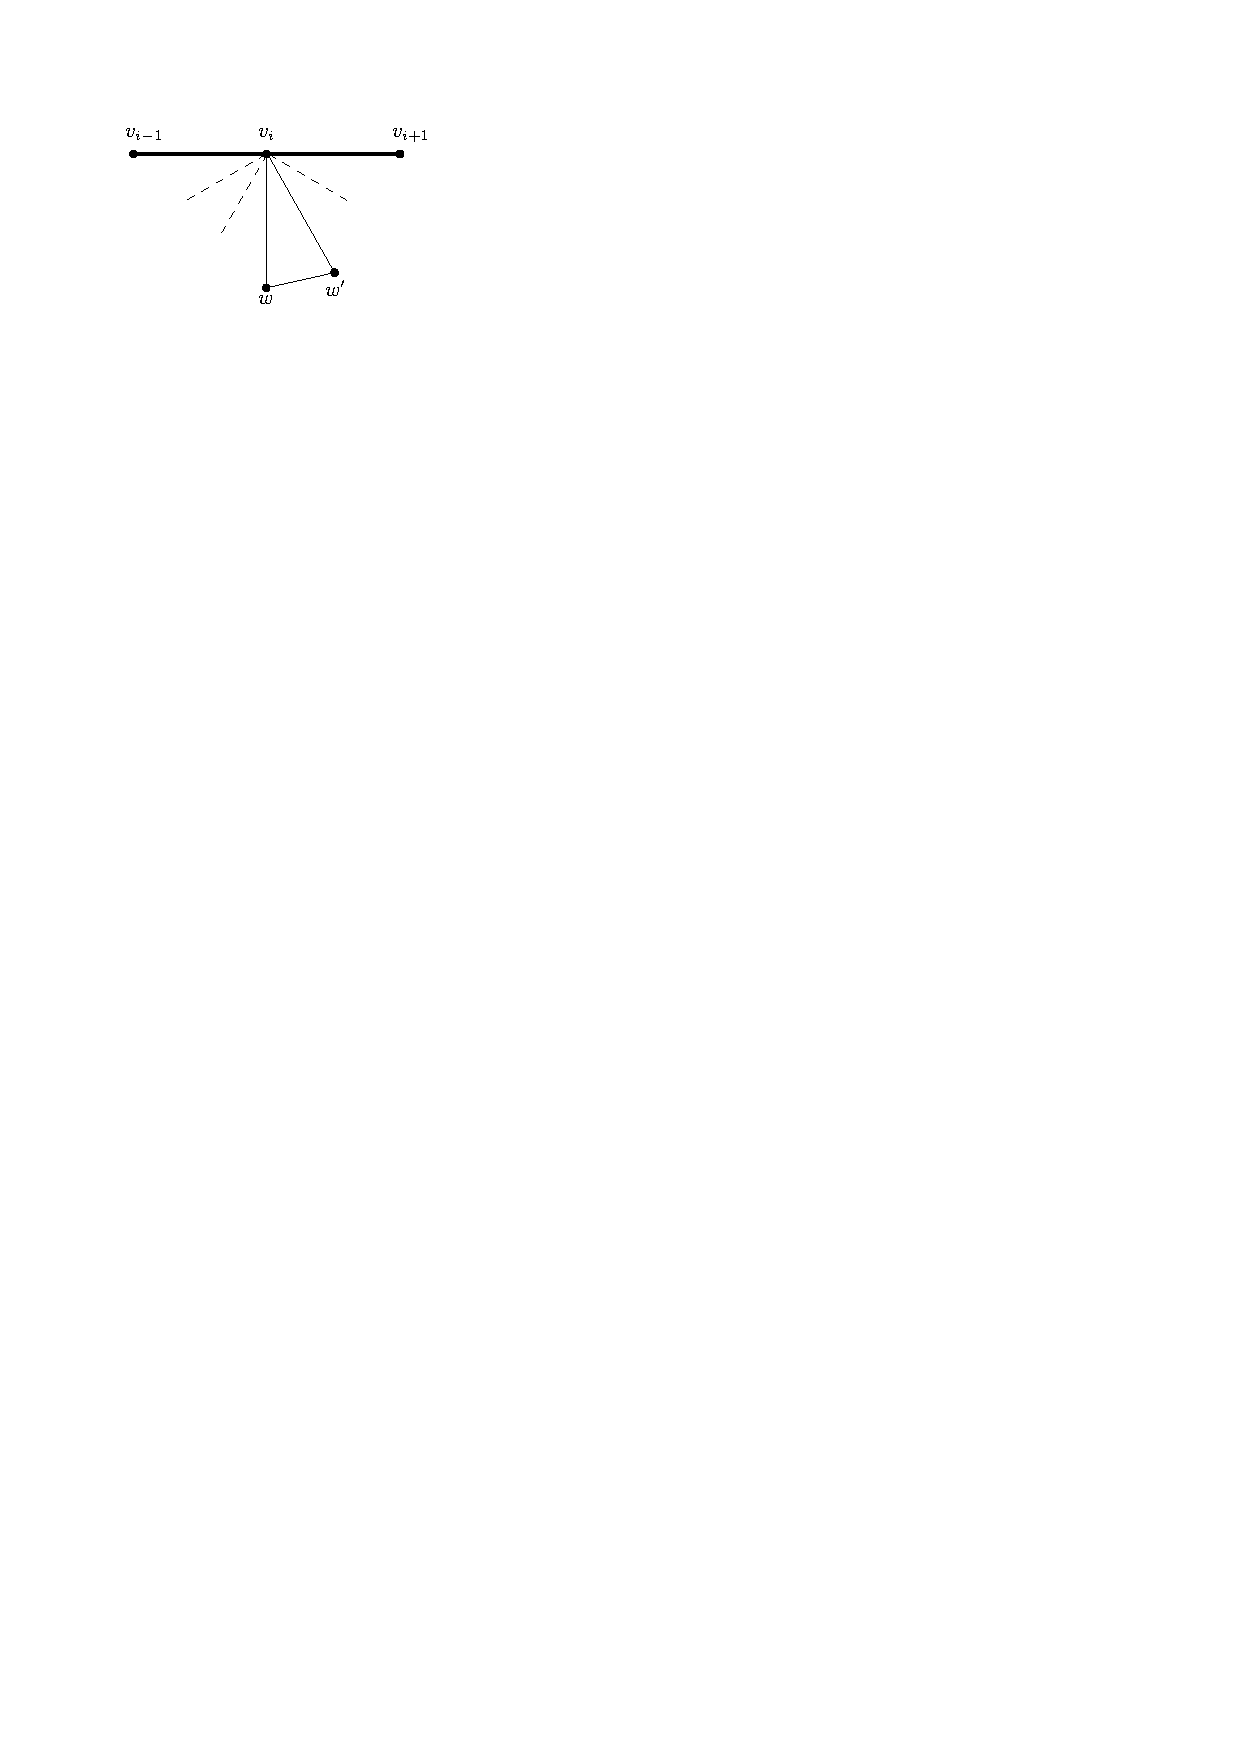
\includegraphics[width=\linewidth]{redAlgo/img/walkProofA}
        \caption{}
    \end{subfigure}%
    \begin{subfigure}[b]{0.5\linewidth}
        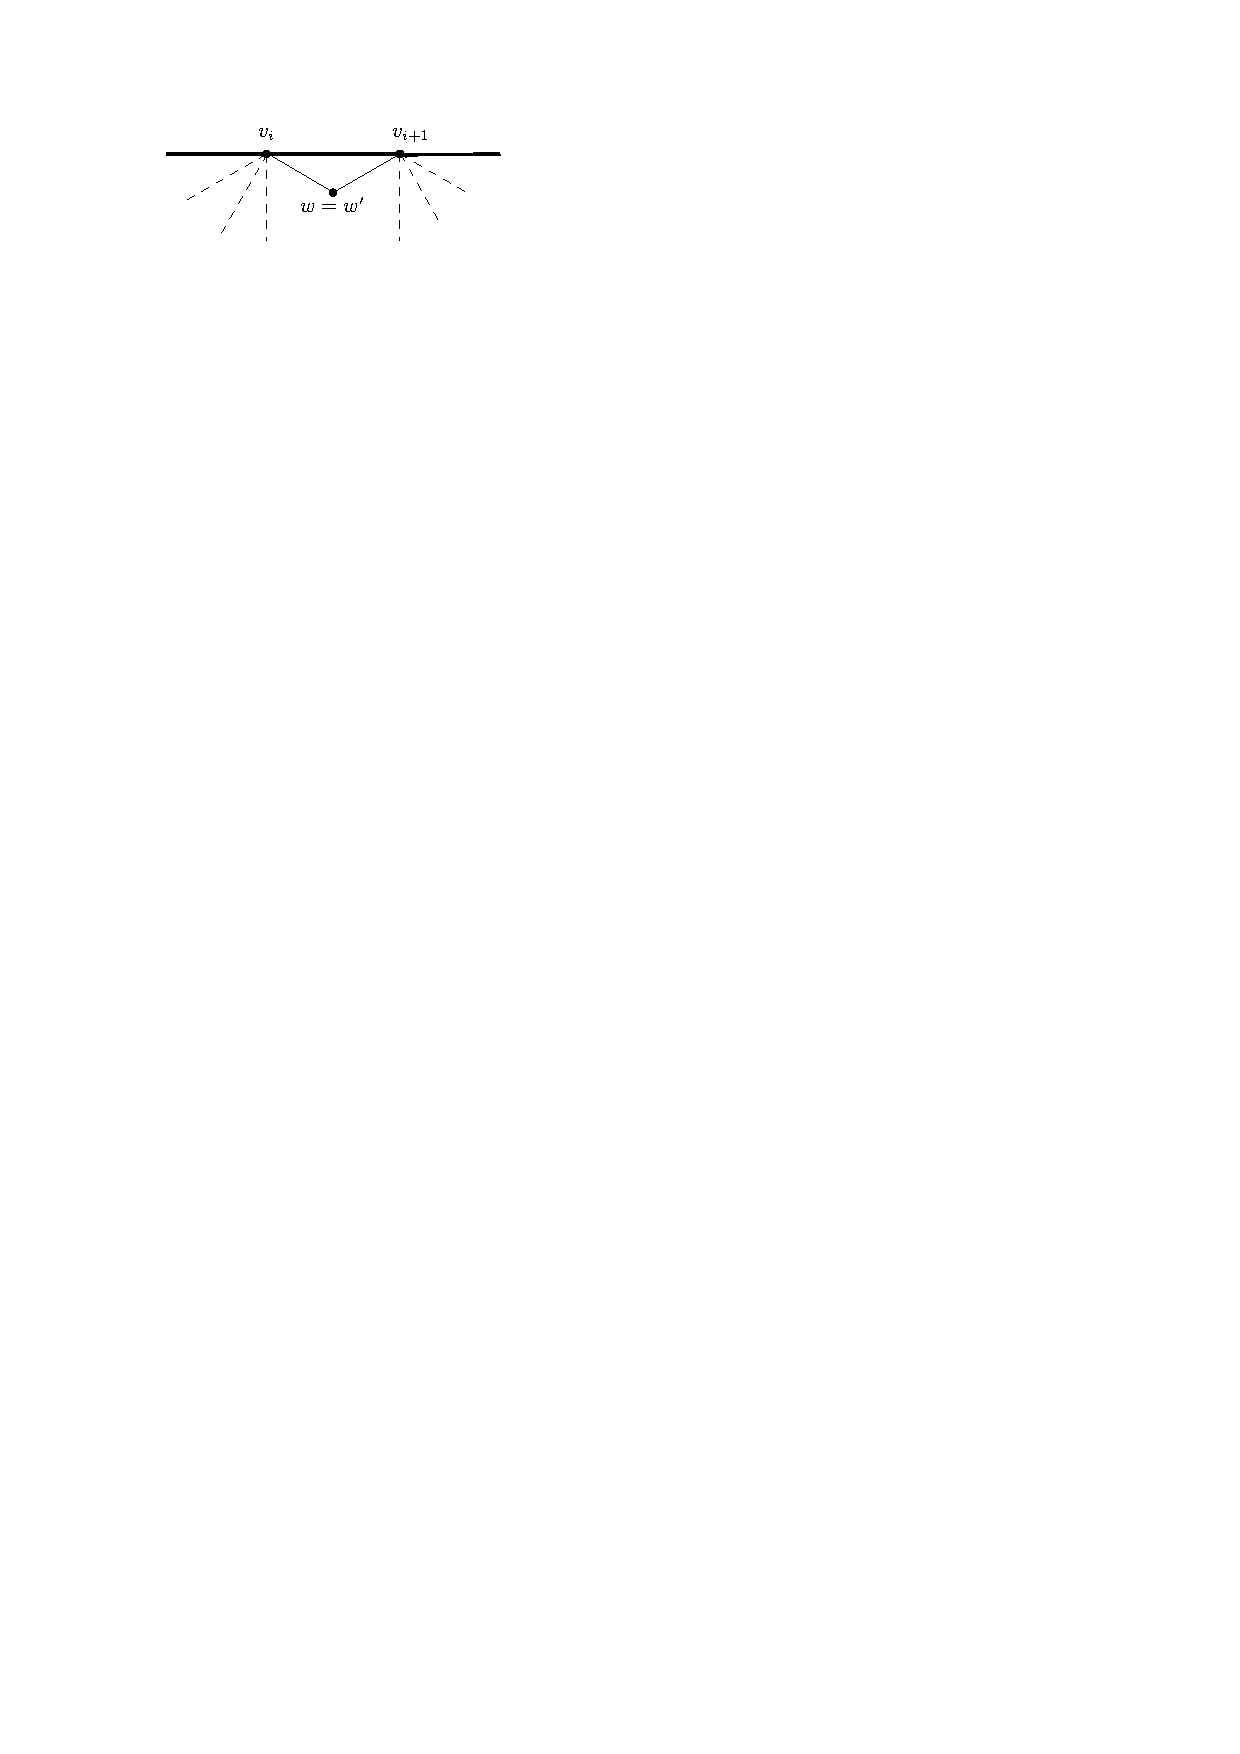
\includegraphics[width=\linewidth]{redAlgo/img/walkProofB}
        \vspace{1cm}

        \caption{}
    \end{subfigure}

    	\caption{The two main cases of the proof showing that $W$ is a walk}
	\label{fig:walkproof}
\end{figure}


In case $(a)$ we note that $v_i w$ and $v_i w'$ are edges next to each other in clockwise order around $v_i$. Since every interior face of $\ext G$ is a triangle $ww'$ must be an edge. We thus see that $w, w'$ are adjacent and not duplicates.

In case $(b)$ we note that $v_i w$ and $v_i v_{i+1}$ are edges subsequent in clockwise order, hence $wv_{i+1}$ is also an edge. Hence $w$ is the first vertex adjacent to $v_{i+1}$ after $v_i$ in clockwise order. Thus $w= w'$. They are duplicates and one of them must have been removed.

Now for the edge cases: Let $w_1$ be the first vertex adjacent to $v_1$ and let $w_m$ be the last vertex adjacent to $v_n$. $\pW$ and $w_1$ are vertices adjacent to $v_1$ subsequent in clockwise order, and hence connected. $w_m$ and $\pE$ are vertices adjacent to $v_n$ subsequent in clockwise order and hence connected.

Hence $\W$ is a walk. The above also shows that $\pW w_1 v_1$ and $\pE v_n w_m$ are triangles and hence $\W$ satisfies properties \ref{p:pW} and \ref{p:pE} of being a prefence.

Moreover this walk satisfies  \ref{p:C} because $\W$ by construction contains all neighbors of any vertex $v_i \in \C \sm{\pW, \pS, \pE}$ between $v_{i-1}$ and $v_{i+1}$ in clockwise order.

Finally to see that $\W$ also satisfies \ref{p:W}. Consider a vertex $w_j \in \W \sm{\pW, \pE}$ then either it is $(a)$ the neighbor of some vertex $v_i$ and only of this vertex or it is $(b)$ the unique vertex neighboring of $\ell +1$ number vertices $v_i, \ldots, v_{i+\ell}$ in the interior of the cycle. This is essentially the same case distinction as above. However now $(a)$ $w_{i-1} w_i v_i$ and $v_i w_i w_{i+1}$ or $(b)$ $w_{i-1} w_i v_i$, $v_i w_i v_{i+1}, \ldots, v_{i+\ell -1} w_i v_{i+\ell} $
 and $v_{i+\ell} w_i w_{i+1}$ form a set of triangles spanning the area between $w_{i-1}$ and $w_{i+1}$ in clockwise order. Thus any edge not going to $\C \sm {\pW, \pS, \pE}$ in this sector will lead to a separating triangle. We however have assumed $G$ has no separating triangles. Hence \ref{p:pW} holds.\footnote{I believe this is still true when separating triangles are allowed to occur. However the prove will have to be different.}
\end{proof}






\subsection{Irregularities}
We will distinguish two kinds of \emph{irregularities} in a prefence.
\begin{enumerate}
\item The candidate walk is non-simple in a certain vertex. That is, if we traverse the sequence of vertices in $\W$ we see that $w_i = w_j$ for some $i<j$.
\item The candidate walk has a chord. That is, there is an edge $w_i w_j$ in $G$ with $i<j$ and $i$ and $j$ not subsequent (i.e. $i < j-1$).

Note that such a chord can only lie on the right of $\W$ ($\W$ being oriented from $\pW$ to $\pE$), since if it would lie on the left of $\W$ the vertices $w_{i+1},\ldots, w_{j-1}$ would not have been chosen by the construction. \fxnote(can we orient a walk like this, maybe make more explicit)
\end{enumerate}

\begin{lemma}
If a prefence has no irregularities it is fence.
\end{lemma}
\begin{proof} \fxnote{refer by labels instead of text}
We will show that all the requirements of being a valid path are met.
 \begin{itemize}
\item [Path] Let us begin by noting that since there are no non-simple points we actually have a path and not just a walk.

\item[\ref{e:noS}] It is clear that both $w_1$ and $w_k$ are not $\pS$ by the construction of the candidate walk.

\item[\ref{e:longBorders}] For $\W$ or $\restC \W$ to have only one edge we need to have that $\pW \pE$ is an edge (since $\W$ is constructed as walk from $\pW$ to $\pE$). However, then one of the $3$-cycles $\pW \pE \pN$ or $\pW \pE \pS$ is separating since the graph $G$ is non-empty. Hence both $\W$ and $\restC \W$ have more than one edge.

\item[\ref{e:crossingEdges}]
We note that $\W$ is both a path and a prefence. Hence \ref{e:crossingEdges} is satisfied. Since every edge with one endpoint on the cycle is of the required type by the conditions of a prefence. Interior edges with both endpoints not on the cycle can a priori exist. However since we have a connected graph there must then also be an edge with  one endpoint in $\C_\W$, but this can not be if $\W$ is a prefence.

\item[\ref{e:noNewChord}] The cycle $\C'$ is simply $\pS \W$ (since $\W$ is  walk from $\pW$ to $\pE$ by construction) and since $\W$ has no chords $\C'$ has none not involving $\pS$.
\end{itemize}
Hence, if $\W$ has no irregularities it is a valid path.

Furthermore, $\W$ is a path from $\pW$ to $\pE$ because it is prefence. And thus
\end{proof}



\begin{defi}[Range of a irregularity]
For a non-simple point \fxnote{Is point the right word? it is def not a vertex} $w_i = w_j$ with $i<j$ has \emph{range} $\braces{i, \ldots, j} \subset \N$.
A chord $w_i w_j$ with $i< j-1$ has \emph{range} $\braces{i, \ldots, j} \subset \N$.
\end{defi}

Note that a chord can't have the same range as a non-simple point since then $w_i w_j$ will be a loop and we are considering simple graphs. Furthermore two chords have different ranges because we otherwise have a multiedge. Two nonsimple points with the same range are, in fact, the same. This leads us to the following remark.
\begin{remark}
\label{rk:diffIregDiffRange}
Different irregularities have different ranges.
\end{remark}

\begin{defi}[Maximal irregularity]
A irregularity is maximal if it's range is not strictly contained\footnote{Because of Remark \ref{rk:diffIregDiffRange} being contained is the same as being strictly contained} in the range of any other irregularity.
\end{defi}

\begin{lemma}
\label{lm:rangeOverlap}
Maximal irregularities have ranges whose overlap is at most one integer.
\fxnote{we might redefine range to make this nicer. However it may make the rest of the algo more ugly. Revisit}
\end{lemma}
\begin{proof}
We let $I$ and $J$ denote two distinct maximal irregularities with ranges $\braces{i_1, \ldots i_2}$ and $\braces{j_1, \ldots, j2}$. Let us for the moment suppose that $I$ and $J$ have ranges that overlap more then one. Since $I$ and $J$ are both maximal their ranges can not be strictly contained in each other and by Remark \ref{rk:diffIregDiffRange} they can't be equal. Hence the ranges must partially overlap.

Without loss of generality we then have $i_1 < j_1 < i_2 < j_2$. Any additional equality in this chain would offend the ranges not being contained in each other or the overlap being larger then one integer.

\fxnote{I need to note somewhere that every vertex in the candidate walk is adjacent to a subpath of $\cpath$}
Now two chords, both laying to the right of $\W$, would cross each other in this case (but we have a planar graph).

A non-simple point $w_{i_1} = w_{i_2}$ is adjacent to two ranges of vertices in $\cpath$. $v_a \ldots v_b$ and $v_c \ldots v_d$ we need that $b$ and $c$ are not subsequent otherwise we have a separating $3$ cycle $w_{i_1} v_b v_c$, now however $\tilde(C) = w_{i_1} v_b \ldots v_c$ is a cycle. And because of the clockwise order of adjacencies around the vertices of $\cpath$ we have that $w_{i_1 +1}, \ldots, w_{i_2 -1}$ are inside this cycle while $ w_1 \ldots w_{i_1 -1}$ and $ w_{i_2 +1} \ldots w_k$ are outside the cycle. See Figure.  \fxfatal{add figure}

Now $J$ being a chord will imply a edge crossing $\tilde{C}$, which can't be. The same argumentation holds symmetrically for $J$ being a non-simple point and $I$ being a chord. Two nonsimple points would imply that the vertex $w_{j_i} = w_{j_2}$ is at the same time inside and outside $\tilde{C}$.
\end{proof}

\subsection{Moves}
\newcommand{\U}{\scr U}
The algorithm will remove these irregularities by recursing on a subgraph for each maximal irregularity. We shrink the cycle $\C$ with every valid path that is found in the recurrence, in the order they are found. Afterwards we update the candidate walk by removing $w_{i+1}, \ldots, w_{j-1}$ in the case of a chord or $w_{i+1}, \ldots, w_{j}$ in the case of a nonsimple point. In subsection \ref{ss:validity} we will show that the updated prefence $\W$ walk is an prefence for the upadated cycle $\C$.


We will first show how to remove these maximal irregularities in Subsections \ref{ss:chords} and \ref{ss:nonsimplePoints}. That is, we show which subgraph $H$ we recurse upon for both kinds of irregularity. Furthermore we show that this subgraph suffices the requirements of the algorithm.

Afterwards, in subsection \ref{ss:validity} we will make sure that the subgraphs we recurse upon are edge-disjoint. That is, they only overlap in border vertices.

It is worth noting that other irregularities contained in such a maximal irregularity are solved in the recurrence.

\subsubsection{Chords}
\label{ss:chords}
If we encounter a chord we will extract a subgraph and recurse on this subgraph. A chord $w_iw_j$ has a triangular face on the left and on the right (like every edge). The third vertex in the face to the left will be called $x$. $x$ is not necessarily distinct from $w_{i+1}$ and/or $w_{j-1}$ but that is also not necessary for the rest of the argument. \fxnote{work out these in a example}

The vertex $v_a$ on the cycle is uniquely determined as the vertices adjacent to both $w_i$ and $w{i+1}$. In the same way $v_b$ is the unique neighbor of $w_{j-1}$ and $w_j$.

We will describe a path $\scr U$ running from $v_a$ to $v_b$. This path consists of all vertices adjacent to $w_i$ in clockwise order from $v_a$ (inclusive) to $x$(inclusive) and subsequently all vertices adjacent to $w_j$ in clockwise order from $x$ (exclusive) to $v_b$ (inclusive). This path is given in bold in Figure \ref{fig:removeChord}.

\fxnote{note this is a walk by a similar argument as $\W$}

\begin{lemma}
$\U$ is a chordfree path
\end{lemma}
\begin{proof}
\fxnote{restructure}
$\U$ cant have a non-simple point $x'$ since it would have to be connected to at least two vertices. However a vertex $x'$ that is distinct from $x$ and is connected to both $w_i$ and $w_j$ will induce a separating triangle $w_i x' w_j$.
\fxnote{make "connected" more precise: connected where?}

$\scr U$ can't have chords $u_i u_j$ since they would either induce a separating $3$- or $4$-cycle either $w_i u_i u_j$ or $w_j u_i u_j$ or $w_i u_i u_j w_j$ depending on the vertex adjacent to $u_i$ and $u_j$.
\fxnote{Here we use no 4-cycles}
\end{proof}


We then consider the interior of the cycle $\C_\scr U$ and the cycle $\C_\U$ itself as the subgraph $H$. We then set $v_a = \pW$ and $v_b = \pE$ and we connect all vertices in $\restC{\U}$ to a new north pole $\pN$ and all vertices in $\U$ to a new south pole $\pS$. We then arrive at the graph $H'$ upon which we will recurse. See also Figure \ref{fig:removeChord}. Since $\C$ is chordfree by invariant \ref{i:noChords} so is $\restC{\U}$. We have also just shown that $\U$ is chordfree. Hence adding the north and south pole doesn't create separating triangles. Furthermore since $H$ is a induced subgraph of $G$ it contains no separating $4$-cycles not involving the poles.

\fxnote{adapt candidate walk}


\begin{figure}[h!]
\centering
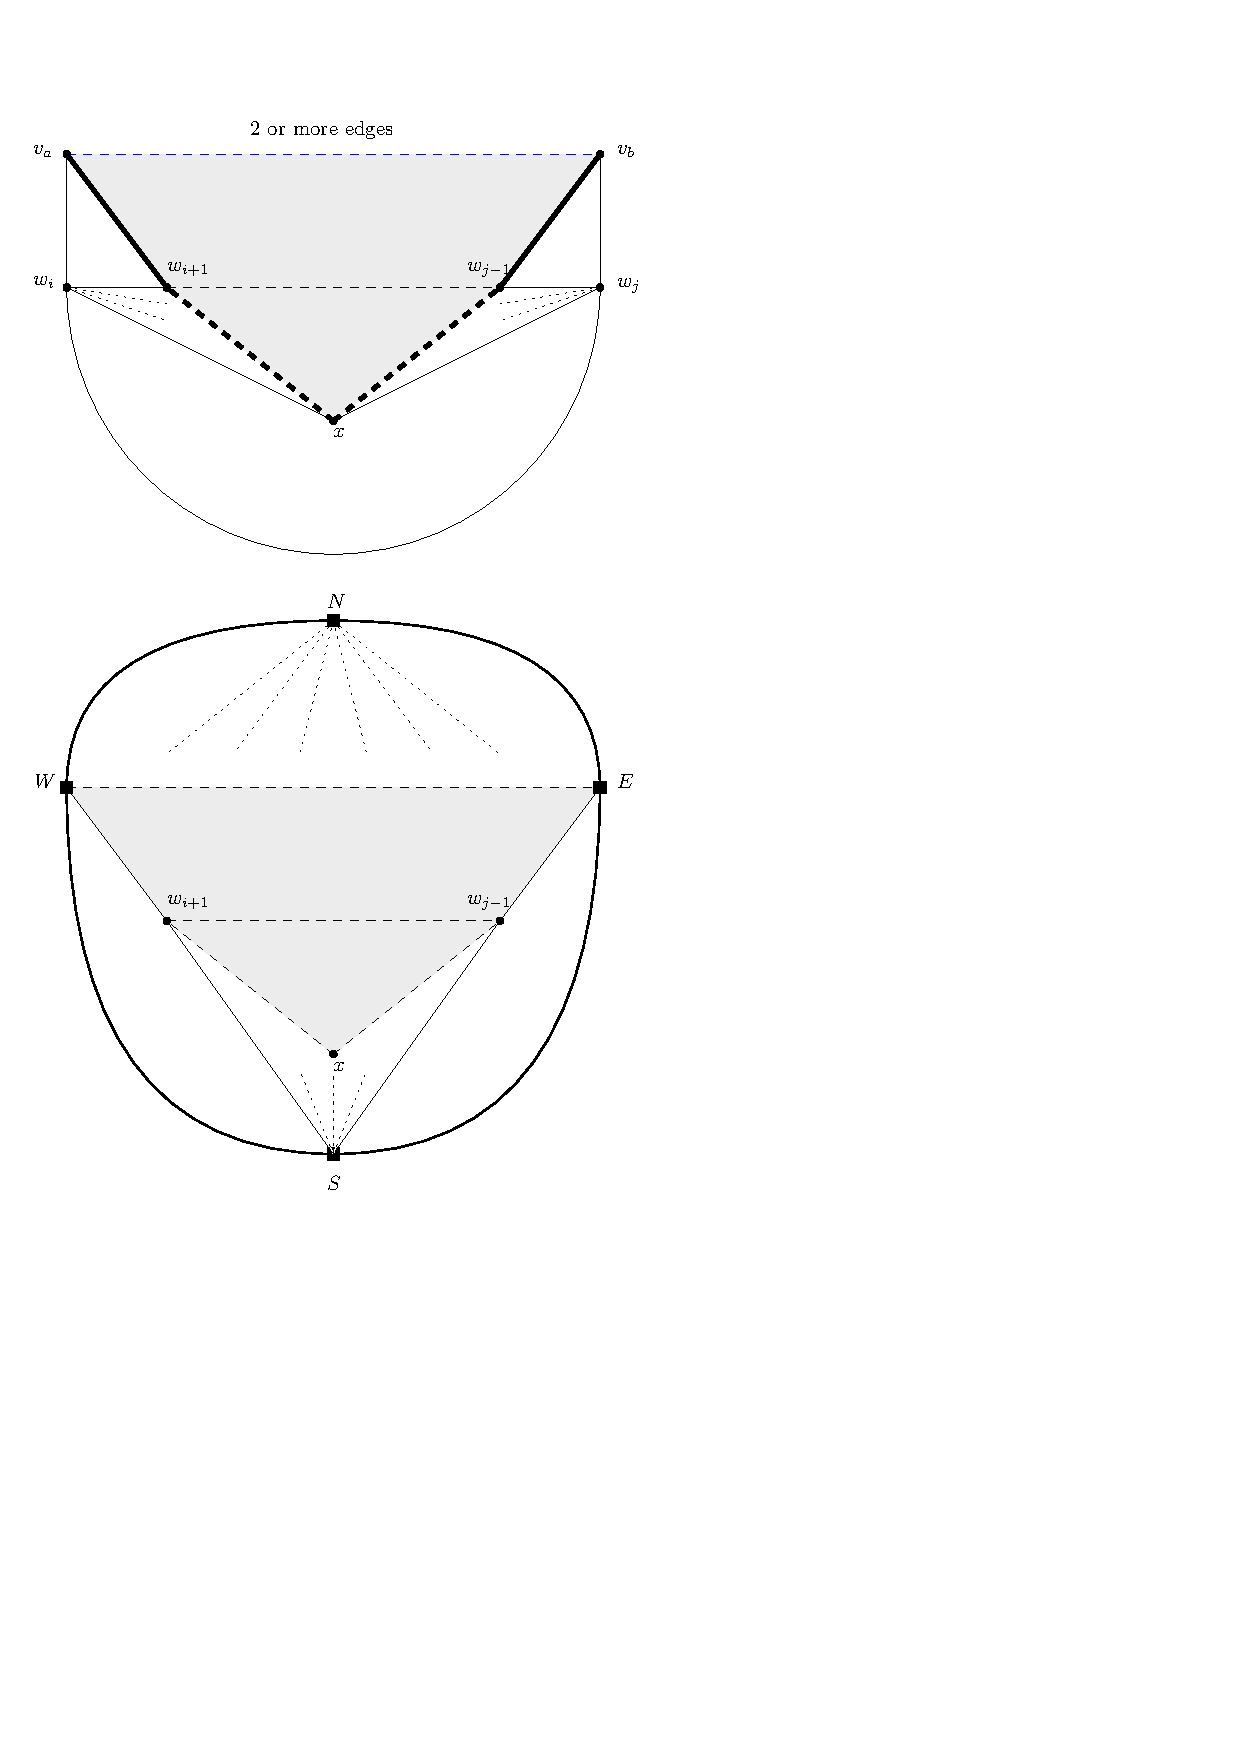
\includegraphics[scale=1]{redAlgo/img/removeChord}

\caption{Removing a chord
    \label{fig:removeChord}}
\end{figure}

\subsubsection{Nonsimple points}
\label{ss:nonsimplePoints}


Removing a non-simple point is done is a similar manner.


The vertex $v_a$ on $\C$ is uniquely determined as the vertices adjacent to both $w_i=w_j$ and $w{i+1}$. In the same way $v_b$ is the unique neighbor of $w_{j-1}$ and $w_j=w_i$. Note that it may be that $w_{i+1} = w{j-1}$ this does not matter for the rest of the argument. \fxnote{show example}

We will describe a path $\scr U$ running from $v_a$ to $v_b$. This path consists of all vertices adjacent to $w_i = w_j$ in clockwise order from $v_a$ (inclusive) to $v_b$(inclusive). This path is given in bold in Figure \ref{fig:removeNonSimplePoint}.

\begin{lemma}
$\U$ is in fact a path, moreover it has no chords.
\end{lemma}
\begin{proof}
\fxnote{restructure}
$\U$ cant have a non-simple point $x$ since such a point would have to be connected to at least two vertices. However every vertex is only connected to $w_i=w_j$.
\fxnote{make "connected" more precise: connected where? On the right of the path}

$\U$ can't have chords on the right of the path by construction. Furthermore $\scr U$ can't have chords $u_i u_j$ on the left since they would either induce a separating $3$-cycle $w_i u_i u_j$.
\fxnote{Here we use no 4-cycles}
\end{proof}


We then consider the interior of the cycle $\C_\scr U$ and the cycle $\C_\U$ itself as the subgraph $H$. We then set $v_a = \pW$ and $v_b = \pE$ and we connect all vertices in $\restC{\U}$ to a new north pole $\pN$ and all vertices in $\U$ to a new south pole $\pS$. We then arrive at the graph $H'$ upon which we will recurse. See also Figure \ref{fig:removeChord}. Since $\C$ is chordfree by invariant \ref{i:noChords} so is $\restC{\U}$. We have also just shown that $\U$ is chordfree. Hence adding the north and south pole doesn't create separating triangles. Furthermore since $H$ is a induced subgraph of $G$ it contains no separating $4$-cycles not involving the poles.

\fxnote{adapt candidate walk}

\begin{figure}[h!]
\centering
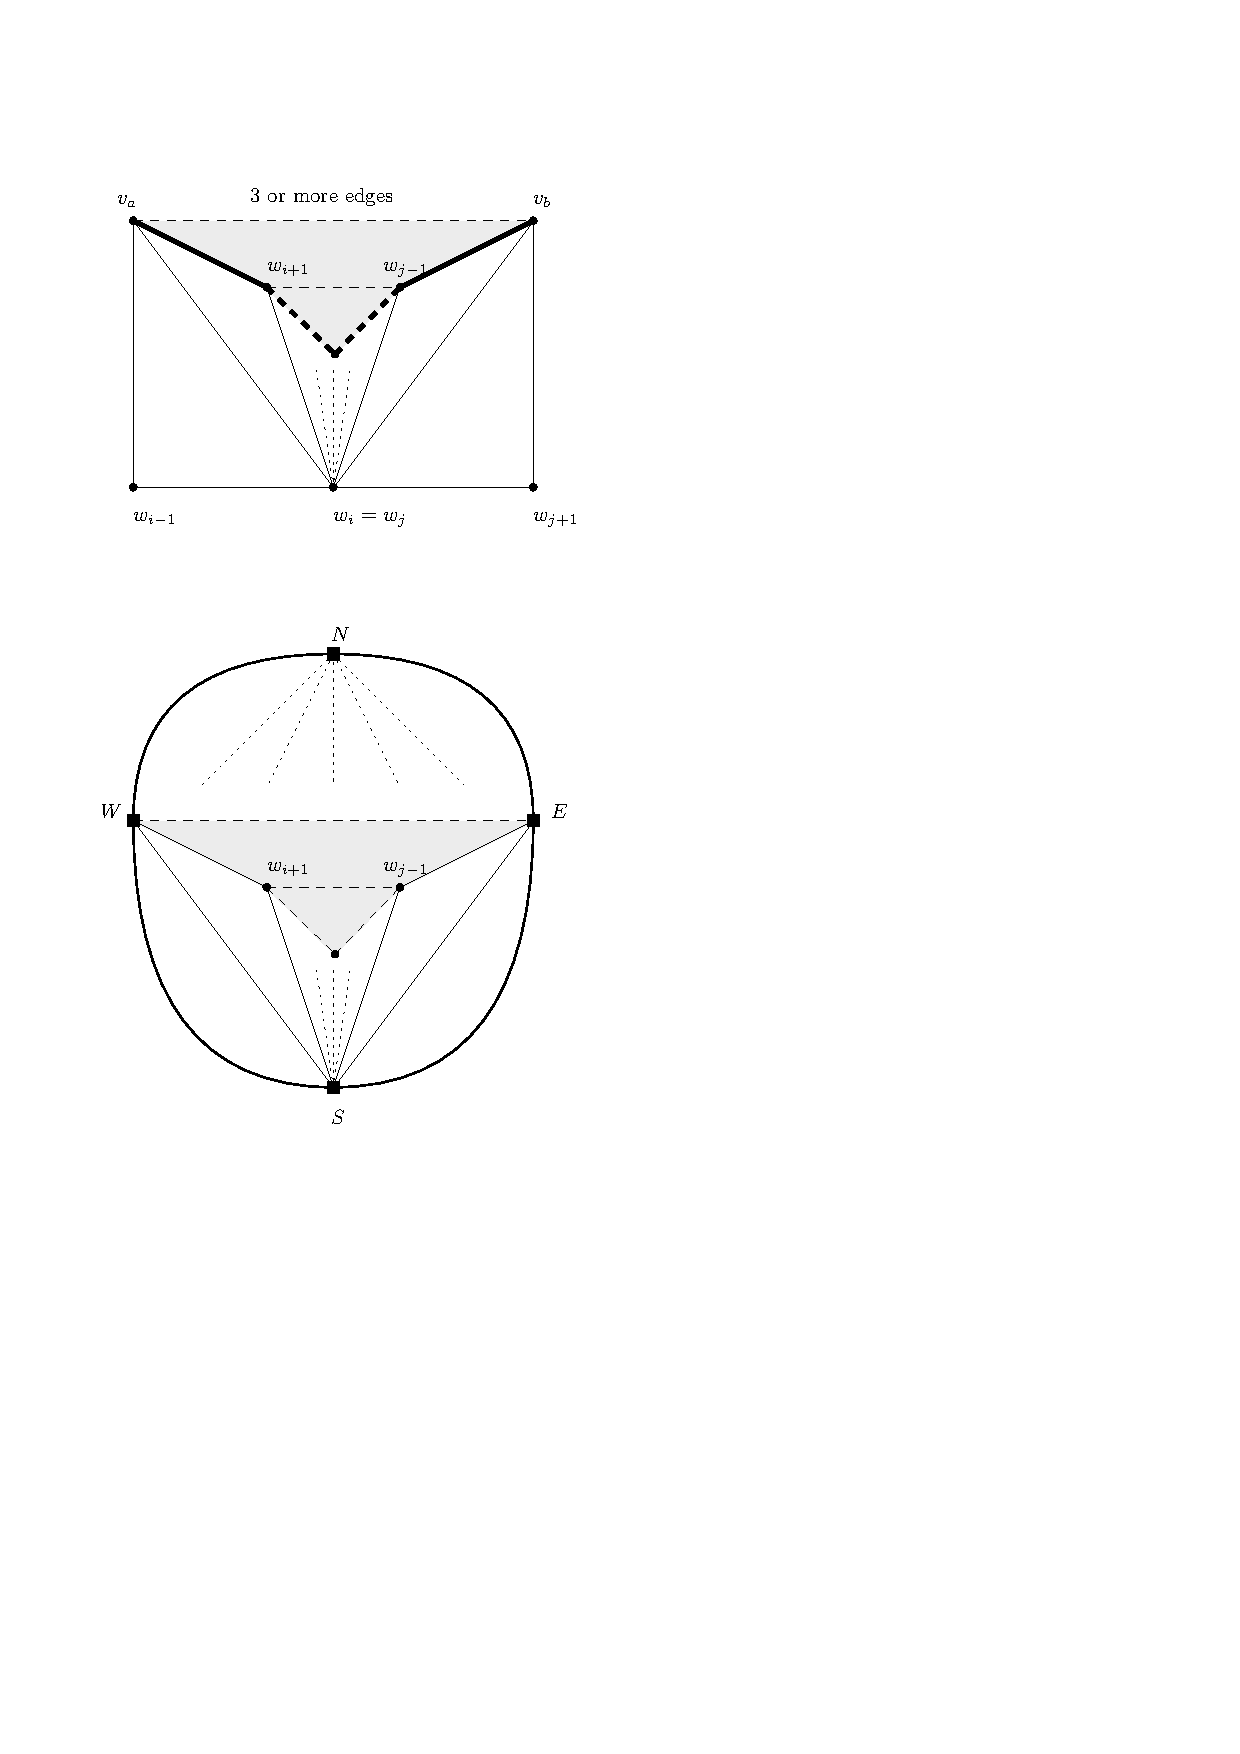
\includegraphics[scale=1]{redAlgo/img/removeNonSimplePoint}

\caption{Removing a non-simple point
    \label{fig:removeNonSimplePoint}}
\end{figure}

\subsubsection{Validity}
\label{ss:validity}

\begin{lemma}
After doing a move the updated prefence $W$ is a prefence for the updated cycle $C$
\end{lemma}
\begin{proof}
\fxerror{TODO}
\end{proof}

\begin{lemma}
Let $H_I$ and $H_J$ be two recursion subgraphs for different maximal irregularities $I$ and $J$. Then $H_I$ and $H_J$ are edge disjoint.
\end{lemma}
\begin{proof}
\fxerror{TODO}
\end{proof}


\subsection{Correctness}
As long as the interior of $\C$ is nonempty we can find

The algorithm finishes because it keeps on recursing and shrinking until no graph is left.

\subsubsection{The red faces}
Let us then argue that the red faces are all $(1-\infty)$ faces, corresponding to one-sided vertical segments.
Let us note that every time we do a move for a maximal irregularity with range $\braces{i, \ldots, j}$. We will shrink the cycle by the valid paths found in the recursion, in the order they are found in the recursion. Insofar these paths are connected to $\C$ they start on or after the unique neighbor of $w_i$ and $w_{i+1}$ on the cycle and the end on or before the unique neighbor of $w_{j-1}$ and $w_j$. Since the ranges of maximal irregularties at most overlap by 1 integer (Lemma \ref{lm:rangeOverlap}) their paths do not overlap


\section{TODO}
Cool examples: The multiple non-simple point $v_i = v_j =v_k$
Example of page $F1$

example with lots of chords
